\documentclass[12pt,a4paper]{article}

% Margins.
\setlength{\oddsidemargin}{0in}
\setlength{\evensidemargin}{0in}
\setlength{\headheight}{12pt}
\setlength{\headsep}{42pt}
\setlength{\topmargin}{-54pt}
\setlength{\textwidth}{6.5in}
\setlength{\textheight}{10in}

\usepackage{amsmath}
\usepackage{float}
\usepackage{graphicx}
\usepackage[hyphens]{url}
\usepackage{hyperref}	% Clickable links to figures, references and urls.
\usepackage{datetime}

% Drawing.
\usepackage{pgf}
\usepackage{tikz}

% Listings for formatting code.
\usepackage{listings}
\usepackage{textcomp}
% General options.
\lstset{breaklines=true, basicstyle=\small\ttfamily, tabsize=4, numbers=left, stepnumber=1, frame=single, showstringspaces=false, upquote=true}
% C++ specific high-lighting. Comments are 50/50 shades of green/black and strings coloured with 60/40 red/black mixture.
\lstset{language=[ISO]C++, commentstyle=\color{green!50!black}, keywordstyle=\color{blue}, stringstyle=\color{red!60!black}}

%opening
\title{\vspace{-3cm}Physics for Engineers\\Assignment 02\\Coordinate Systems, Surfaces and Integrals}
\author{Arshad Hassan\and Attique Dawood}
\date{September 04, 2013\\Due: September 11, 2013\\[0.2cm] Last Modified: \today, \currenttime}
\begin{document}
\maketitle
\noindent\textbf{Question 1:} Do the following point conversions.
\begin{itemize}
\item[(a)] (-1, 2, -3) to cylindrical and spherical coordinates.
\item[(b)] (3, 35$^0$, -2) to cartesian and spherical coordinates.
\item[(c)] (2, 105$^0$, 190$^0$) to cartesian and cylindrical coordinates.
\end{itemize}
\noindent\textbf{Question 2:} Sketch and describe the following surfaces.
\begin{itemize}
\item[(a)] $\rho=1$
\item[(b)] $\phi=30^0$
\item[(c)] $r=5$
\item[(d)] $\theta=30^0$
\item[(e)] $\rho=1$, $0<\phi<\pi$ and $0<z<4$
\item[(f)] $r=1$, $0<\theta<\pi/2$ and $0<\phi<2\pi$
\item[(g)] $r=1$, $0<\theta<\pi/2$ and $0<\phi<\pi/2$
\end{itemize}
\noindent\textbf{Question 3:} Using $\int_{a}^{b}\hat n\cdot d\textbf{\textit{l}}$
\begin{itemize}
\item[(a)] Find the length of line segment from (0, 0) to (1, 2). Solve this in Cartesian as well as Cylindrical coordinates.
\item[(b)] Find the length of body/space diagonal of a unit cube.
\item[(c)] Find the arc length of a quarter circle of radius $\rho=3$ m in first quadrant.
\item[(d)] Find the length of the curve $y=x^2$ from (0, 0) to (1, 1). For this problem a calculator would be handy in solving the integrals.
\item[(e)] Find the length of the curve $y=2x^2+2$ from (0, 2) to (2, 10).
\end{itemize}
\noindent\textbf{Note:} For part (d) you need to find a unit vector along the curve $y=x^2$. A vector parallel (or tangent) to $y=x^2$ can be obtained from the slope. Numerator and denominator of slope ($\dfrac{dy}{dx}$) are the $y$-- and $x$--components, respectively, of the vector. Here, $\dfrac{dy}{dx}=\dfrac{2x}{1}$ so the parallel/tangent vector is $\textbf{n}=\hat x+2x\hat y$. The unit vector is then $\hat n=\dfrac{\hat x+2x\hat y}{\sqrt{1+4x^2}}$.\\[0.2cm]
\newpage
\noindent\textbf{Question 4 (Example 2--4C \cite[Example 2--4, page 23]{Cheng}):} Given a force field $\textbf{F}=xy\hat x+(3x-y^2)\hat y$ in a region, evaluate the integral $\int_{P1}^{P2}\textbf{F}\cdot d\textbf{\textit{l}}$ to find the total work done in moving from P1 to P2 along path 1 and path 2.\\[0.2cm]
\noindent\textbf{Question 5:} Electric field in a region is $\textbf{E}=x\hat x+y\hat y$. Refer to figure \ref{Cheng-integral}, evaluate the integral $\int_{P1}^{P2}\textbf{E}\cdot d\textbf{\textit{l}}$ to find the potential difference between P1 and P2. Is the potential difference same for path 1 and path 2?
\begin{figure}[H]
\centering
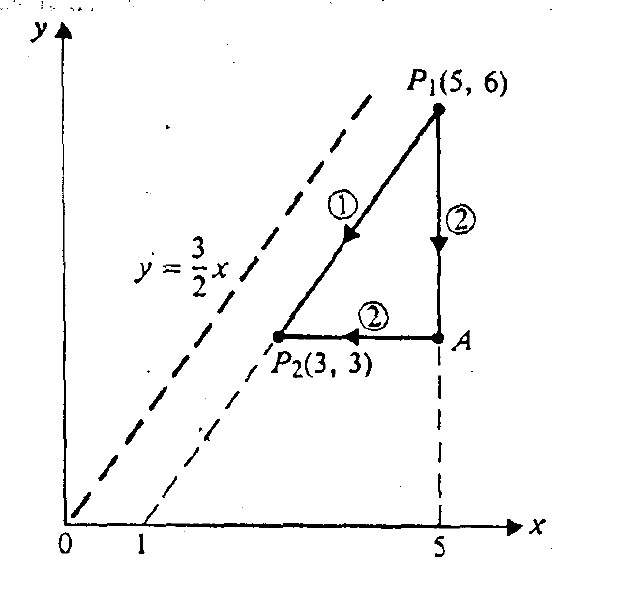
\includegraphics[scale=0.6]{Figure2-10Cheng.png}
\caption{Paths of integration for Question 2 \cite[Figure 2--10, page 23]{Cheng}}
\label{Cheng-integral}
\end{figure}
\noindent\textbf{Question 6:} Do the following end--of--chapter problems from reference book \cite[Page 93 and 94]{Sadiku}: 3.1, 3.2, 3.3 and 3.7.
%\nocite{*}
\bibliographystyle{plain}
\bibliography{PhysicsRef}
\end{document}
